\phantomsection
%\addcontentsline{toc}{chapter}{Introduzione}
\chapter{GreenCloud Simulator Overview}
\markboth{GreenCloud Simulator Overview}{}
% [titolo ridotto se non ci dovesse stare] {titolo completo}

\begin{citazione}
In this chapter the reason for the selection of \emph{GreenCloud} simulator as the reference tool for the simulations will be explained. Then several aspects about \emph{GreenCloud} will be covered, including its usage, its source code and the output files of the simulations.

\end{citazione}
\newpage

\section{Selection of \emph{GreenCloud}} 
Based on the comparisons made among the different analyzed simulators, each of them has its strengths and weaknesses. However, for the needs required in the study addressed by this thesis work, it is essential to prioritize aspects related to the energy consumption of the Data Center and the accuracy of simulations. From the conducted comparisons, it is evident that \emph{GreenCloud} is the simulator that accurately considers these aspects as it is built on top of the \emph{NS2} simulator and fully implements the \emph{TCP/IP} protocol. Moreover, \emph{GreenCloud} offers its users a set of features related to the simulation and to the energy consumption management. In particular, it is possible to choose between several pre-implemented Data Center architectures and energy models as well as to customize them. Furthermore, \emph{GreenCloud} provides various workload scheduling and power saving models, allowing programmers to implement new ones. Despite \emph{GreenCloud} simulation times tend to be high, for the purposes of this study it is reasonable to prioritize granularity over performance. Therefore, the study will continue using \emph{GreenCloud} as the reference tool for the simulations to be conducted. The following sections provide a description of various aspects of \emph{GreenCloud} based on the work by \emph{Kliazovich et al.} \cite{kliazovich2012greencloud}.

\section{\emph{GreenCloud} project}
In the following subsections, two aspects of the \emph{GreenCloud} simulator project will be covered, namely the simulator source code structure and the description of the output files that are generated upon simulation completion.  
\subsection{Simulator source code} \label{subsection:greencloud_code}
The \emph{GreenCloud} source code is organized into three directories: \emph{dashboard}, \emph{ns2/greencloud}, and \emph{scripts}:
\begin{itemize}
\item \emph{dashboard} contains \emph{HTML}, \emph{CSS}, and \emph{JS} code related to the simulation report page;
\item \emph{ns2/greencloud} contains \emph{C++} code that implements the core functionalities of the simulator, the energy models of the Data Center components, scheduling algorithms, and energy-saving models;
\item \emph{scripts} includes various \emph{TCL} and \emph{Bash} scripts that facilitate the modification of simulation parameters and allows to create simulation reports.
\end{itemize}
Since the scripts in the \emph{scripts} directory require access to various variables within the \emph{C++} classes to modify and read them for constructing logs, each class associates each variable with a symbolic name using the \emph{bind} method. This allows the scripts to access these variables.
For instance, the class \emph{DcHostClass} defined in \emph{ns2/greencloud/dchost.cc} exposes several variables related to a Data Center host, including the current load, current energy consumption, and the total consumed energy.

\subsection{Simulation input parameters}
The executed simulations are highly customizable by users. Below are descriptions of some of the most important parameters along with the files in which they can be modified:
\begin{itemize}
    \item \textbf{SCHEDULER}: specifies the scheduling algorithm used. The available options are: \emph{Green} \emph{RoundRobin}, \emph{Random}, \emph{HEROS}, \emph{RandDENS} and \emph{BestDENS}. This parameter can be set at line 9 of the \href{https://github.com/vincenzo-emanuele/masters-degree-thesis/tree/main/greencloud\_modified\_src/run.sh}{run.sh} script;
    \item \textbf{TOPOLOGY}: indicates the type of Data Center architecture. The possible choices are \emph{three-tier}, \emph{three-tier high-speed}, \emph{three-tier debug}, \emph{three-tier heterogenous debug} and \emph{three-tier heterogenous}. Although \emph{GreenCloud}-related literature mentions a two-tier architecture implementation, such implementation is not found in the simulator's source code. This parameter can be set at line 10 of the \href{https://github.com/vincenzo-emanuele/masters-degree-thesis/tree/main/greencloud\_modified\_src/run.sh}{run.sh} script;
    \item \textbf{top(NCloudUser)}: specifies the number of Data Center users. It can be set at line 11 of the \href{https://github.com/vincenzo-emanuele/masters-degree-thesis/blob/main/greencloud_modified_src/scripts/user.tcl}{user.tcl} script;
    \item \textbf{serv(eDVFS\_enabled)} and \textbf{serv(eDNS\_enabled)}: indicate the usage of \emph{DVFS} and \emph{DNS} in Data Center servers. These can be set at lines 19 and 20 of the \href{https://github.com/vincenzo-emanuele/masters-degree-thesis/blob/main/greencloud\_modified\_src/scripts/setup\_params.tcl}{setup\_params.tcl} script;
    \item \textbf{switches(eDVFS\_enabled)} and \textbf{switches(eDNS\_enabled)}: indicate the usage of \emph{DVFS} and \emph{DNS} in Data Center switches. These can be set at lines 28 and 29 of \href{https://github.com/vincenzo-emanuele/masters-degree-thesis/blob/main/greencloud\_modified\_src/scripts/setup\_params.tcl}{setup\_params.tcl};
    \item \textbf{task(mips)}, \textbf{task(memory)}, \textbf{task(storage)}, \textbf{task(size)}, \textbf{task(duration)}, \textbf{task(outputsize)}, and \textbf{task(intercom)}: indicate various properties of tasks to be executed. In particular, \emph{task(mips)} signifies the required computation in \emph{MIPS}, \emph{task(memory)} indicates required \emph{RAM} in bytes, \emph{task(storage)} denotes required storage memory in bytes, \emph{task(duration)} specifies the computing deadline in seconds, \emph{task(outputsize)} represents the length of output upon task completion in bytes, and \emph{task(intercom)} describes the size of inter-task communication. These parameters can be set at lines 67-82 of \href{https://github.com/vincenzo-emanuele/masters-degree-thesis/blob/main/greencloud\_modified\_src/scripts/setup\_params.tcl}{setup\_params.tcl}.



\end{itemize}

\subsection{Simulation output files} \label{subsection:simulationoutput}
At the end of a simulation, \emph{GreenCloud} generates various report files in \emph{TR} format, that provide a detailed exploration of different aspects of the conducted simulations. Specifically, the following files are produced:
\begin{itemize}
    \item \emph{dcLoad.tr:} a time-stamped log of the Data Center load throughout the entire simulation;
    \item \emph{dcLoadMem.tr:} a time-stamped log of the Data Center memory load throughout the entire simulation;
    \item \emph{dcLoadStor.tr:} a time-stamped log of the Data Center storage load throughout the entire simulation;
    \item \emph{dcPower.tr:} a time-stamped log of the power consumed by servers;
    \item \emph{dcServLoad.tr:} it reports the average load for each server during the simulation;
    \item \emph{dcServLoadMem.tr:} it reports the average memory load for each server during the simulation;
    \item \emph{dcServLoadStor.tr:} it reports the average storage load for each server during the simulation;
    \item \emph{dcServTasks.tr:} it reports the average number of submitted tasks per server;
    \item \emph{dcServTasksFailed.tr:} it reports the average number of failed tasks per server;
    \item \emph{dcVmLoad.tr:} it reports the average load for each \emph{VM} during the simulation;
    \item \emph{dcVmLoadMem.tr:} it reports the average memory load for each \emph{VM} during the simulation;
    \item \emph{dcVmLoadStor.tr:} it reports the average storage load for each \emph{VM} during the simulation;
    \item \emph{dcVmTasks.tr:} it reports the average number of submitted tasks for each \emph{VM} during the simulation;
    \item \emph{dcVmTasksFailed.tr:} it reports the average number of failed tasks for each \emph{VM} during the simulation;
    \item \emph{eAccessSwitches.tr:} it reports the amount of energy consumed by each access layer switch during the simulation;
    \item \emph{eAggrSwitches.tr:} it reports the amount of energy consumed by each aggregation layer switch during the simulation;
    \item \emph{eCoreSwitches.tr:} it reports the amount of energy consumed by each core layer switch during the simulation;
    \item \emph{energySummary.tr:} it reports the amount of energy consumed by all switches during the simulation;
    \item \emph{eServers.tr:} it reports the amount of energy consumed by each server during the simulation;
    \item \emph{link\_C1C2\_load.tr:} it reports the average load on network links connecting core switches to aggregation switches in the downlink;
    \item \emph{link\_C2C1\_load.tr:} it reports the average load on network links connecting aggregation switches to core switches in the uplink;
    \item \emph{link\_C2C3\_load.tr:} it reports the average load on network links connecting aggregation switches to Top-of-Rack (\emph{ToR}) switches in the downlink;
    \item \emph{link\_C3C2\_load.tr:} it reports the average load on network links connecting Top-of-Rack (\emph{ToR}) switches to aggregation switches in the uplink;
    \item \emph{link\_C3H\_load.tr:} it reports the average load on network links connecting computing servers to thier Top-of-Rack (\emph{ToR}) switches in the downlink;
    \item \emph{link\_HC3\_load\_time.tr:} it reports the average load on network links connecting computing servers to thier Top-of-Rack (\emph{ToR}) switches in the uplink; 
    \item \emph{link\_HC3\_load.tr:} it reports the load dynamics of a single link connecting a given server to its Top-of-Rack (\emph{ToR}) switch in the uplink; 
    \item \emph{loadSummary.tr:} it reports the Data Center average load;
    \item \emph{parameters.tr:} it contains a summary of the input simulation parameters;
    \item \emph{queue\_C3C2-0\_pkts.tr:} it reports the queue size in packets on network links connecting Top-of-Rack (\emph{ToR}) switches to aggregation switches in the uplink;
    \item \emph{queue\_HC3\_pkts\_avg.tr:} it reports the average queue size in packets on network links connecting computing servers to their Top-of-Rack (\emph{ToR}) switches in the uplink;
    \item \emph{queue\_HC3\_pkts\_time.tr:} it reports the queue load dynamics in packets of a single link connecting a given server to its Top-of-Rack (\emph{ToR}) switch in the uplink;
    \item \emph{serv\_load\_time.tr:} a time-stamped log of the servers load throughout the entire simulation;
    \item \emph{simulation.tr:} it reports the simulation duration;
    \item \emph{taskSummary.tr:} it reports a summary of executed and failed tasks;
    \item \emph{users.tr:} it reports several Data Center users statistics.
\end{itemize}
The information about these files is obtained from the descriptions provided in the \emph{dashboard/graph-definitions.js} file. To access a more immediate summary of the conducted simulations, the \emph{dashboard/dashboard.html} file can be viewed using a web browser. This webpage presents essential simulation details along with various charts, as illustrated in figures \ref{fig:greencloud_energy} and \ref{fig:greencloud_overall}. 
\begin{figure}[h]
    \centering
    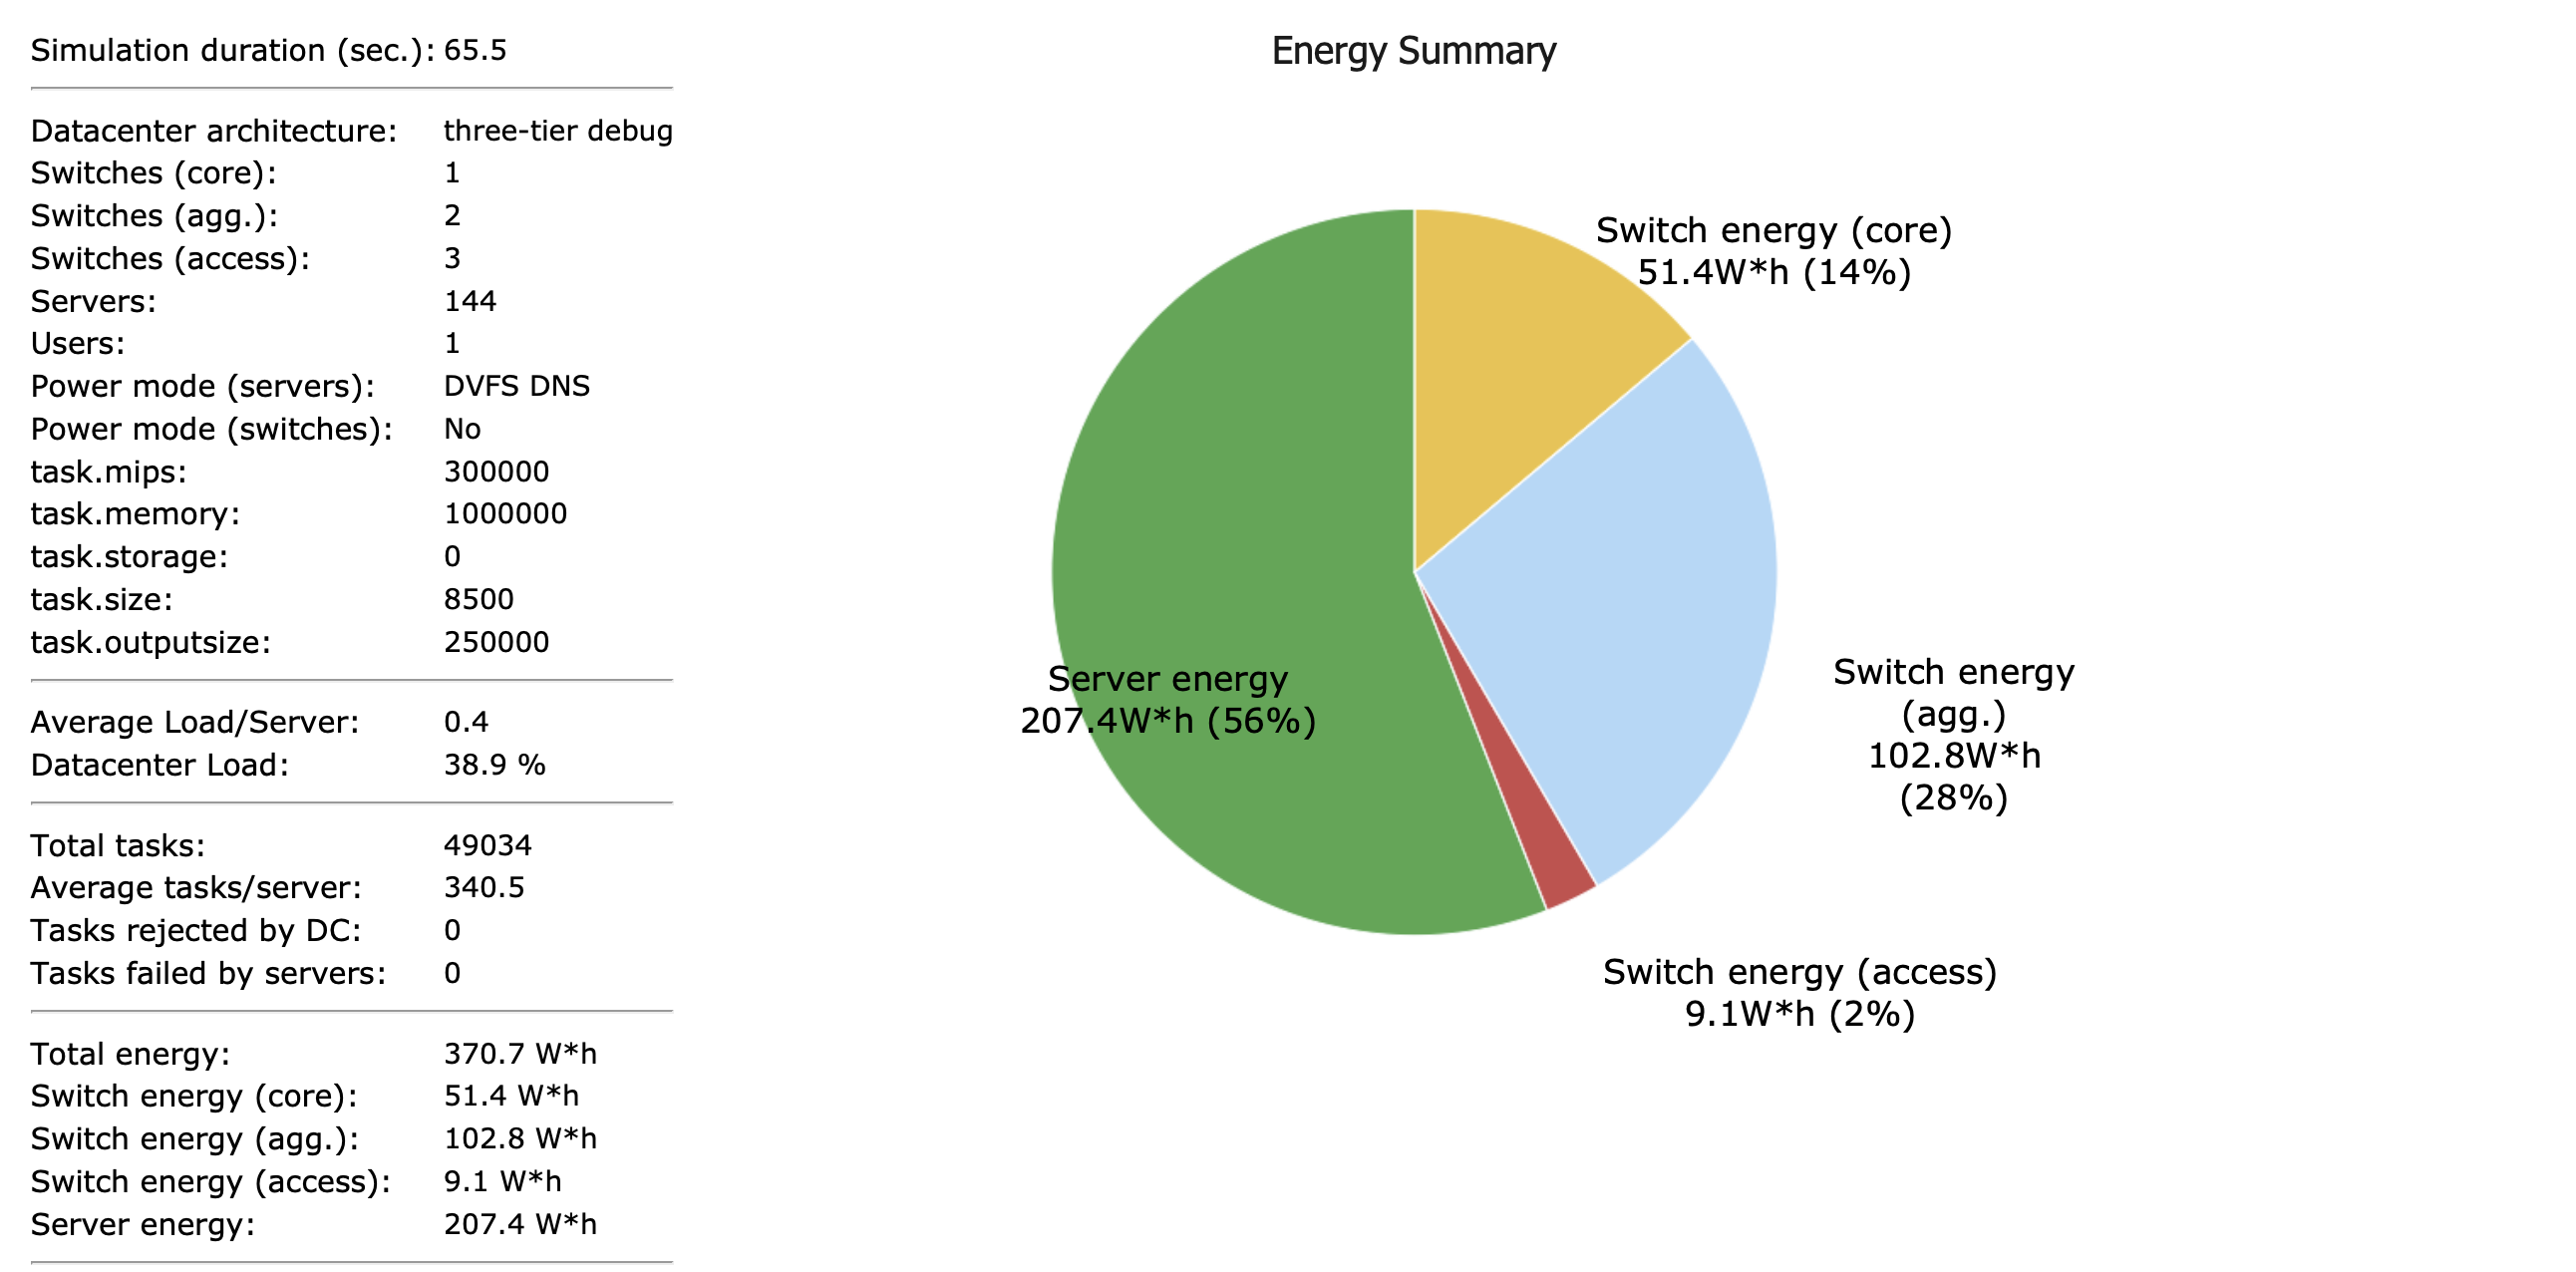
\includegraphics[width=0.8\textwidth]{chapters/images/greencloud_energy.png}
    \caption{\emph{GreenCloud} energy consumption chart}
    \label{fig:greencloud_energy}
\end{figure}

\begin{figure}[h]
    \centering
    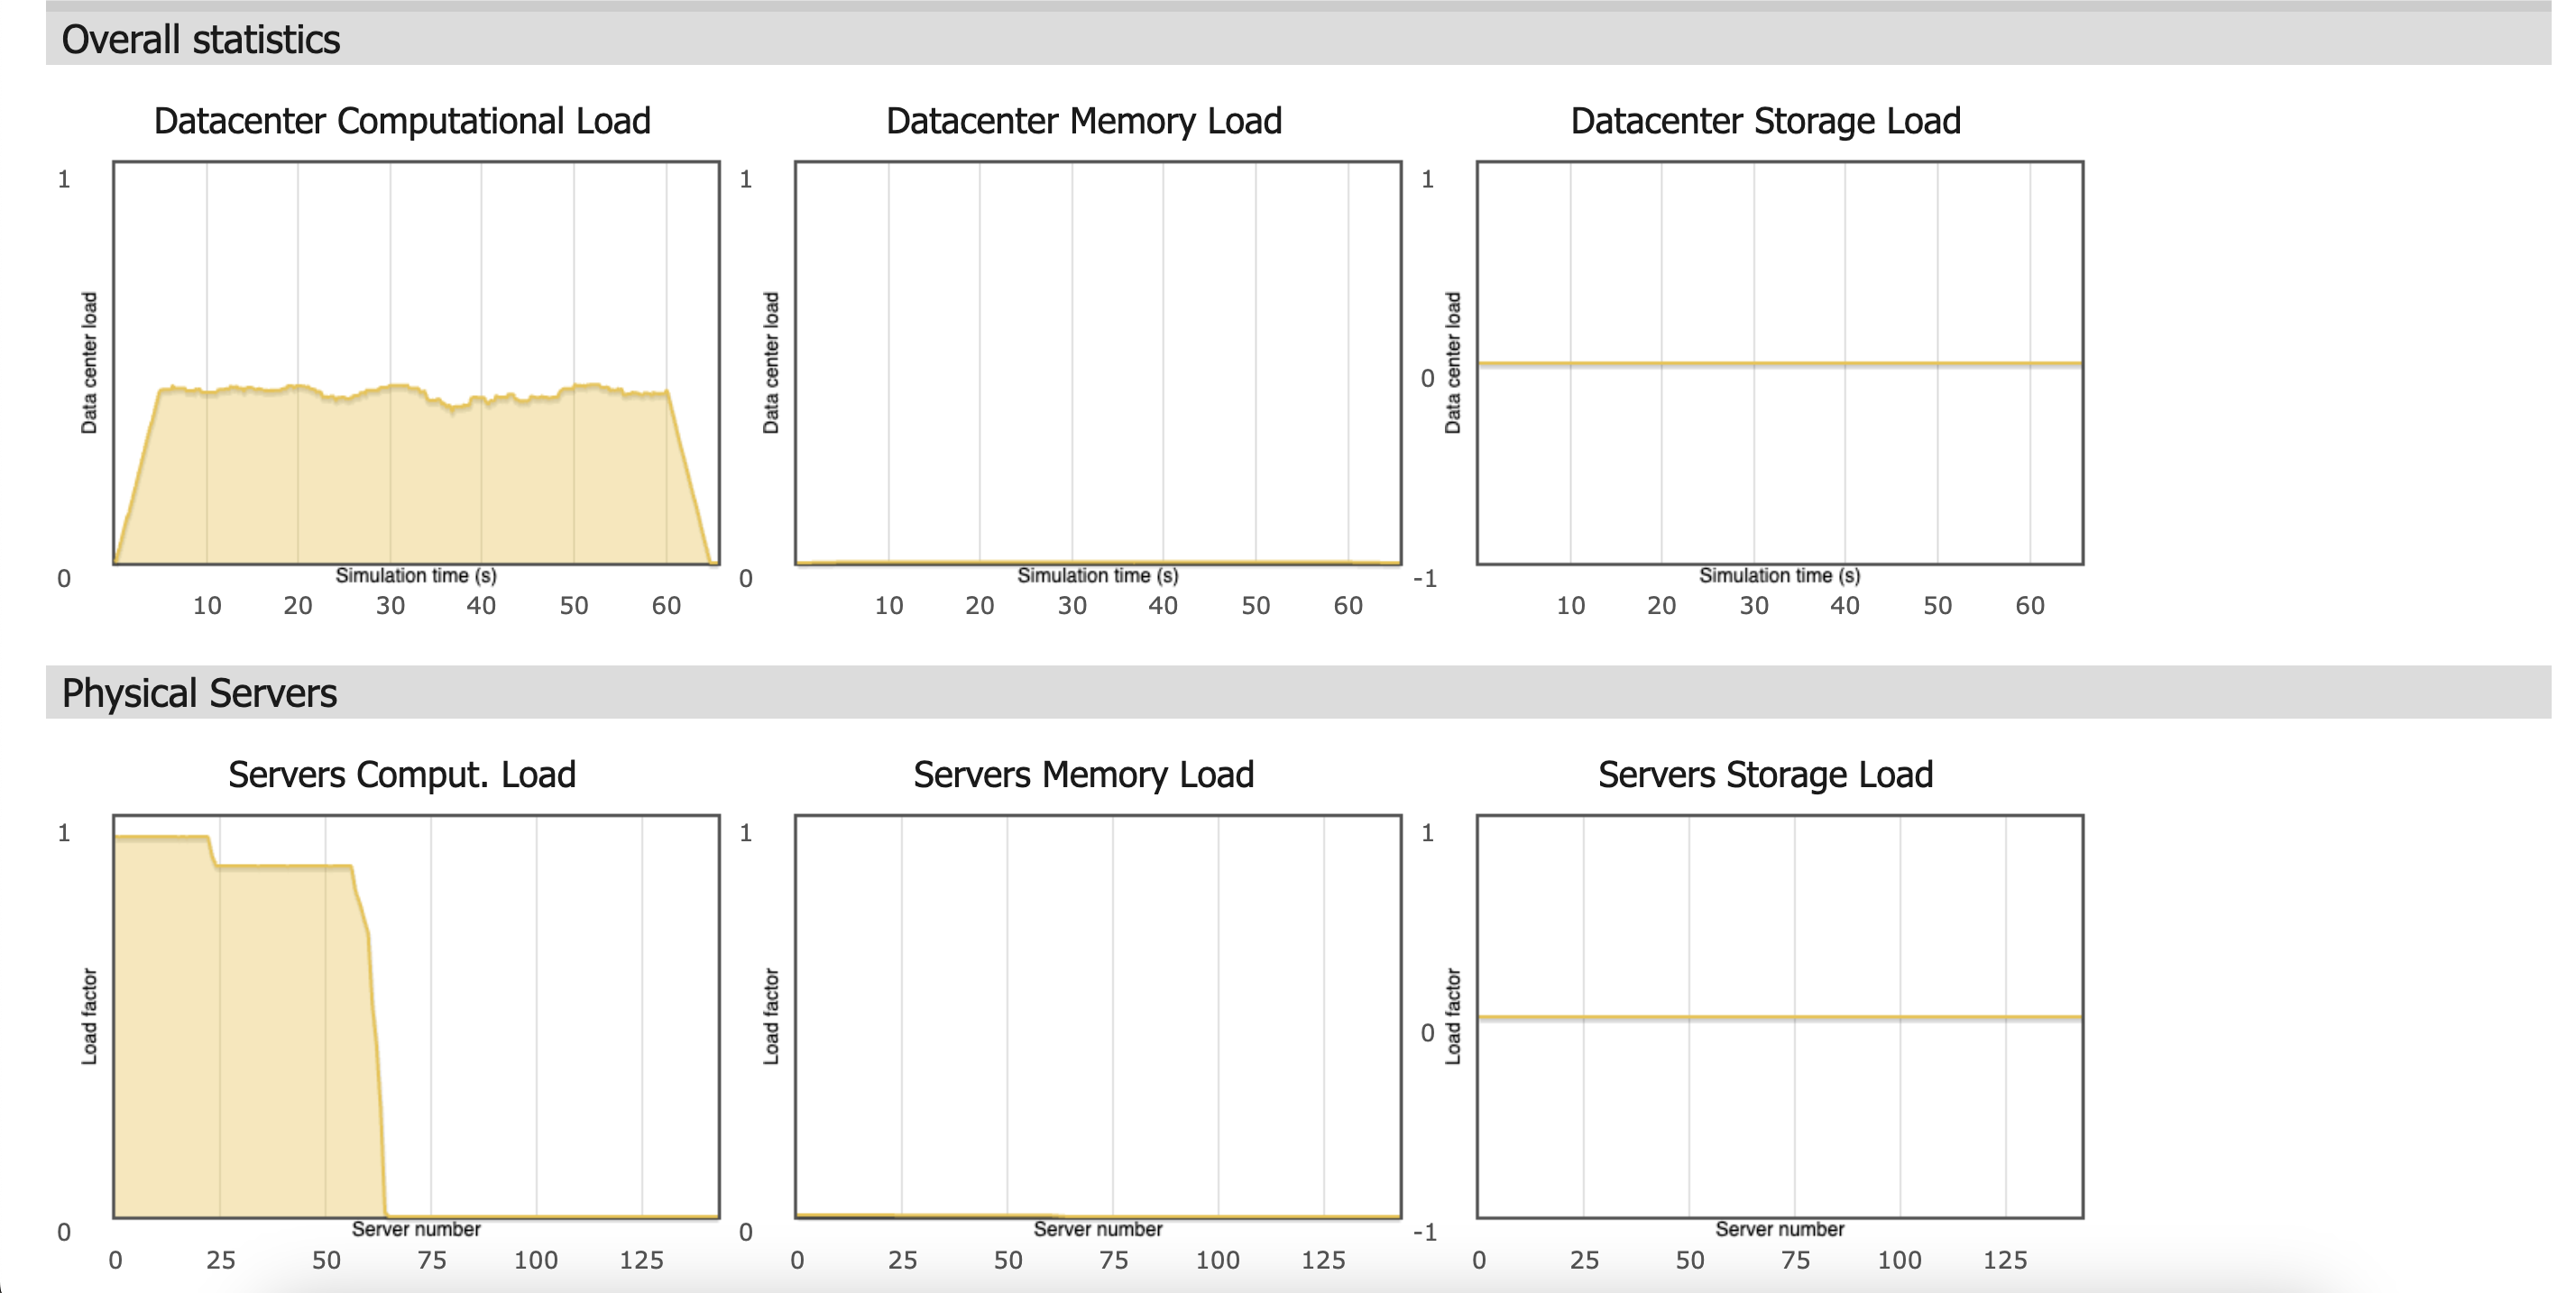
\includegraphics[width=0.8\textwidth]{chapters/images/greencloud_overall.png}
    \caption{\emph{GreenCloud} overall statistics charts (partial)}
    \label{fig:greencloud_overall}
\end{figure}
\section{Available Data Center architectures} \label{chapter:architectures}
As mentioned in the previous section, \emph{GreenCloud} provides several Data Center architectures. The implemented architectures consist of various components, described as follows:
\begin{itemize}
    \item \textbf{Servers:} single core nodes with a fixed processing power limit expressed in \emph{MIPS} (million instructions per second) or \emph{FLOPS} (floating point operations per second) that are responsible for task execution. These components are organized in racks and the architecture includes the presence of a Top-of-Rack switch that connects them to the access layer of the architecture;
    \item \textbf{Switches and links:} they implement the interconnection between the Servers in the Data Center. The type and the quality of these devices influences the transmission rate, anyway the costs of such devices need to be taken into account. Switches usually support either 1 \emph{GE (Gigabit Ethernet)} or 10 \emph{GE} as transmission rates, while links usually support 10 \emph{Mb/s}, 100 \emph{Mb/s}, and 1 \emph{Gb/s} as transmission rates;
    \item \textbf{Workloads:} the representation of tasks to be executed that consist of two components, computational and communicational. The computational part specifies the required amount of computing resources, measured in \emph{MIPS} or \emph{FLOPS}, and the duration of resource allocation. On the other hand, the communicational component of the workload entails the quantity and dimensions of data transfers essential before, during, and after the workload execution.
\end{itemize}
The following subsections provide an overview of the available Data Center architectures within the \emph{GreenCloud} simulator. Since, as mentioned in the previous chapter, this simulator is based on \emph{NS2}, it is possible to customize the Data Center architecture. 

\subsubsection{Two-tier Data Center architecture}
Two-tier architecture is shown in figure \ref{fig:greencloud_twotier}. This architecture consists of an \emph{Access Network} layer where rack switches group several computing Servers through 1 \emph{GE} links and a \emph{Core Network} layer where \emph{L3} switches provide full mesh connectivity through 10 \emph{GE} links. This type of architecture supports up to 5500 nodes.
\begin{figure}[h]
    \centering
    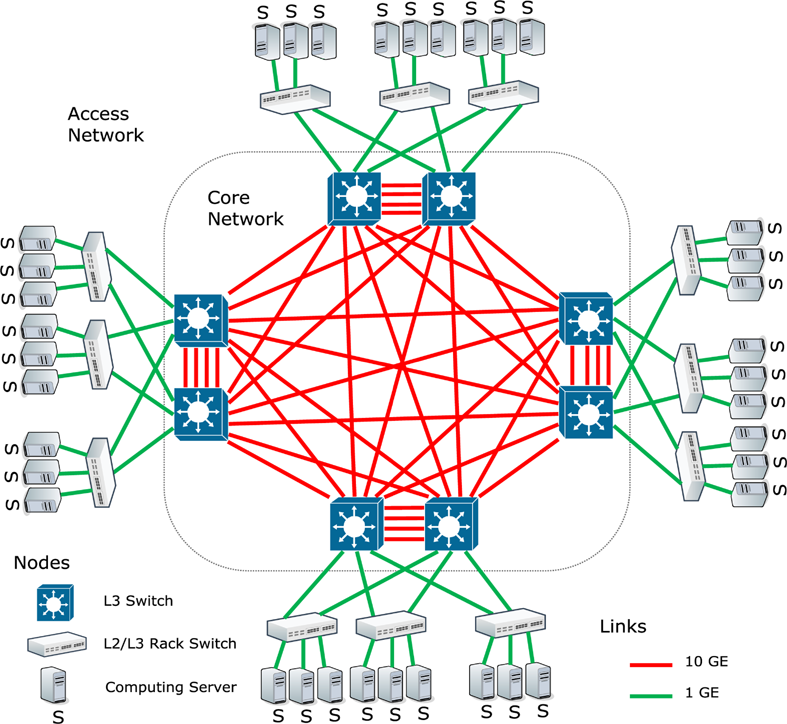
\includegraphics[width=0.5\textwidth]{chapters/images/greencloud_twotier.png}
    \caption{\emph{GreenCloud} two-tier architecture}
    \label{fig:greencloud_twotier}
\end{figure}

\subsubsection{Three-tier Data Center architecture}
Three-tier architecture is shown in figure \ref{fig:greencloud_threetier}. This architecture consists of an \emph{Access Network} layer where rack switches group several computing Servers through 1 \emph{GE} links, an \emph{Aggregation Network} and a \emph{Core Network} where \emph{L3} switches provide full mesh connectivity through 10 \emph{GE} links. This type of architecture is the most commonly used nowadays.

\begin{figure}[h]
    \centering
    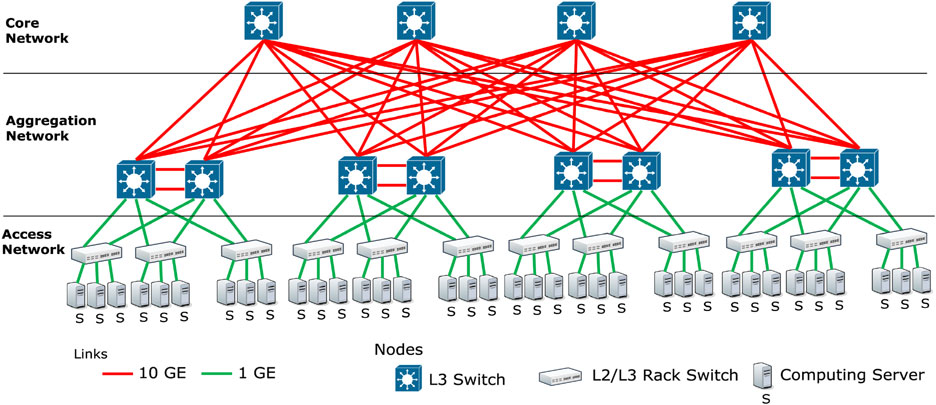
\includegraphics[width=0.7\textwidth]{chapters/images/greencloud_threetier.png}
    \caption{\emph{GreenCloud} three-tier architecture}
    \label{fig:greencloud_threetier}
\end{figure}

\subsubsection{Three-tier high-speed Data Center architecture}
Three-tier high-speed architecture is shown in figure \ref{fig:greencloud_threetierhs}. This architecture is analogous to the three-tier architecture except it employs 100 \emph{GE} links in the \emph{Aggregation Network} and \emph{Core Network} instead of 10 \emph{GE} ones. Moreover, it consists of only two \emph{L3} Switches in the \emph{Core Network} instead of four.
\begin{figure}[h]
    \centering
    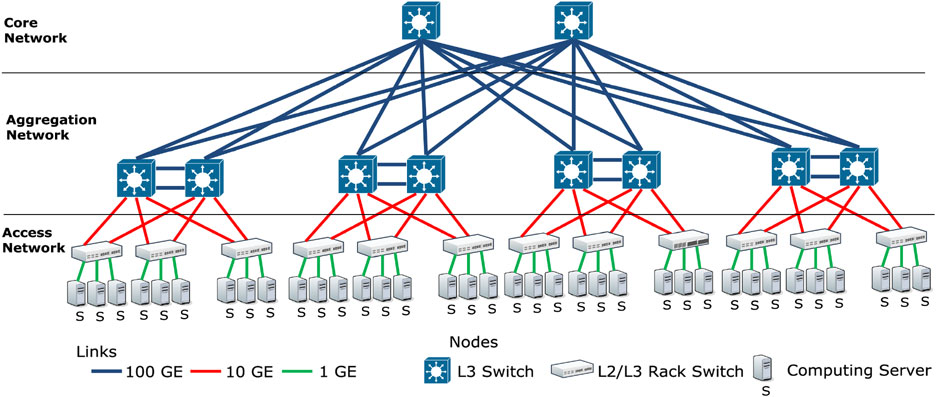
\includegraphics[width=0.7\textwidth]{chapters/images/greencloud_threetierhs.png}
    \caption{\emph{GreenCloud} three-tier high-speed architecture}
    \label{fig:greencloud_threetierhs}
\end{figure}

\section{Available power saving models}
Two power saving models are available within the \emph{GreenCloud} simulator, namely \emph{Dynamic Voltage and Frequency Scaling (DVFS)} which makes the energy consumption of servers proportional to their operating frequency and \emph{Dynamic Network Shutdown (DNS)} which places idle servers into a sleep mode. The power savings achieved through these techniques are not negligible. According to \cite{kliazovich2012greencloud} the use of \emph{DVFS} results in a power savings of 4\%, the use of \emph{DNS} leads to a savings of 63\%, and the combined use of both techniques results in a savings of 65\%. It is evident that the most significant contribution comes from the utilization of \emph{DNS}, as an active server consumes a considerable amount of energy that does not scale with the operating frequency.

\section{Energy model of servers, switches, memory and disks}
Since \emph{GreenCloud} aims to be suitable for energy management, the authors provided the energy models related to the components of the Data Center architecture. The following subsections present the energy models described in \cite{kliazovich2012greencloud} for each described component.
\subsubsection{Servers}
Assuming that \(f\) is the operating frequency of the \emph{CPU}, \(P_{fixed}\) is the fixed energy consumption that does not scale with \(f\) and \(P_f\) is the \emph{CPU}-dependent energy consumption, the total energy consumption of a server is calculated as follows (equation \ref{eq:server_energy}):
\begin{equation} \label{eq:server_energy}
    P_{server} = P_{fixed} + P_f \cdot f^3
\end{equation}
\subsubsection{Switches}
The power consumption model for switches is illustrated in \cite{makaratzis2018energy} and is described by the following equation (equation \ref{eq:switch_energy}):
\begin{equation} \label{eq:switch_energy}
    P_{switch} = P_{chassis} + n_cP_{linecard} + \sum_{r=1}^{R} n^r_pP^r_pu^r_p,
\end{equation}
where \(P_{chassis}\) is the energy consumed by the switch hardware, \(n_c\) is the number of line cards, \(n_p^r\) is the number of ports running at rate \(r\),  \(P_{linecard}\) is the energy consumed by a linecard, \(P_p^r\) is the energy consumed by a port running at rate \(r\) and \(u_p^r\) represents a port utilization, defined as follows (equation \ref{eq:port_utilization}):
\begin{equation} \label{eq:port_utilization}
    u_p = \frac{1}{T} \int_{t}^{t+T} \frac{B_p(t)}{C_p} dt = \frac{1}{T\cdot C_p} \int_{t}^{t+T} B_p(t) dt,
\end{equation}
where \(B_p(t)\) is an instantaneous throughput at the port's link at the time \(t\), \(C_p\) is the link capacity, and \(T\) is a measurement interval. 
\subsubsection{Memory and disks}
\emph{GreenCloud} implements a simple energy model for memory and disks as it allows to choose between the idle and the maximum power of these components resulting respectively in the minimum and the maximum consumption. 

\section{Workload scheduling algorithms} 
The choice of the scheduling algorithm significantly affects the energy consumption of the Data Center. As previously mentioned, \emph{GreenCloud} provides various scheduling algorithms and, due to its open-source nature, allows developers to create new ones. This section provides an overview of the algorithms available within the simulator and conducts a comparison among them.
\subsection{Algorithms description}
The \emph{GreenCloud} simulator provides the following scheduling algorithms:
\begin{itemize}
    \item \textbf{Green:} this energy-aware scheduler groups the workload onto the fewest number of computing servers possible;
    \item \textbf{RoundRobin:} it cyclically distributes the tasks across a set of servers for a fixed time slice. Once the time elapses, this scheduler moves to the next task;
    \item \textbf{Random:} it allocates tasks by randomly choosing servers;
    \item \textbf{RAND-DENS and BEST-DENS:} they aim to reduce the energy usage of the Data Center by choosing the most suitable computing resources for tasks execution. This selection is based on two parameters, namely the load level and the communication potential of Data Center components, defined as the available end-to-end bandwidth that specific servers or groups of servers can access through the Data Center \cite{kliazovich2013dens};
    \item \textbf{HEROS:} it allocates tasks to a server based on a score computed through a decision function based on two subfunctions, namely the \emph{server selection function} and the \emph{communication potential function}. The \emph{server selection function} is based on the idea that the power usage of different hardware can vary a lot in terms of how much energy it uses and how it behaves, while the \emph{communication potential function} is similar to the \emph{DENS} communication potential function but it uses the actual link load instead of the queue buffer size \cite{guzek2015heros}.
\end{itemize}
\subsection{Algorithms comparison}
In order to evaluate the performance of these algorithms, several simulations were performed using \emph{GreenCloud}. These simulations model\ the scenario where a specific amount of computational work is requested by a certain number of users and fulfilled by a specific number of servers within a given timeframe. In particular, all simulations have been executed with the same parameters described below:
\begin{itemize}
    \item \textbf{Architecture:} a three-tier debug architecture was utilized, differing only from the three-tier architecture described in Section \ref{chapter:architectures} in terms of the number of components comprising the Data Center. Specifically, 144 servers, 3 switches at the access layer, 2 switches at the aggregation layer, and one switch at the core layer were employed;
    \item \textbf{Number of users:} due to simulation time constraints, only two users were instantiated;
    \item \textbf{Processing power (MIPS):} the total processing power required by the tasks to be executed amounts to 600000 \emph{MIPS};
    \item \textbf{Simulation time:} the simulation models a scenario in which the servers process client requests for 60 seconds;
    \item \textbf{Adopted power saving models:} the power saving model adopted for switches is \emph{DVFS}, while for servers both \emph{DVFS} and \emph{DNS} were employed.
\end{itemize}
The \href{https://github.com/vincenzo-emanuele/masters-degree-thesis/tree/main/scheduling\_algorithms\_comparison/simulations}{reports} provided by \emph{GreenCloud} regarding these simulations can be found on the \emph{GitHub} \href{https://github.com/vincenzo-emanuele/masters-degree-thesis}{repository} related to this research work, where each directory contains the files generated for each scheduling algorithm. Furthermore, an \emph{xlsx} file has been generated, containing a time-stamped log of the overall energy consumption and \emph{PUE} of the Data Center throughout the entire simulation, for each described scheduling algorithm. In order to calculate the time-stamped log of the energy consumption, it was necessary to make specific modifications to the simulator code, which will be adequately detailed in Section \ref{section:greencloud_mod}. Additionally, computing the Power Usage Effectiveness (\emph{PUE}) involved the utilization of an external tool, discussed further in Subsection \ref{subsection:powercooling}. In order to provide an immediate understanding of the behavior of these aforementioned algorithms, three charts (one for energy consumption, one for \emph{PUE} and one that summarizes the total energy consumed during the simulation) have been produced (figures \ref{fig:schedulers_energyconsumption}, \ref{fig:schedulers_pue} and \ref{fig:schedulers_totalconsumption}). \\
\begin{figure}[h]
    \centering
    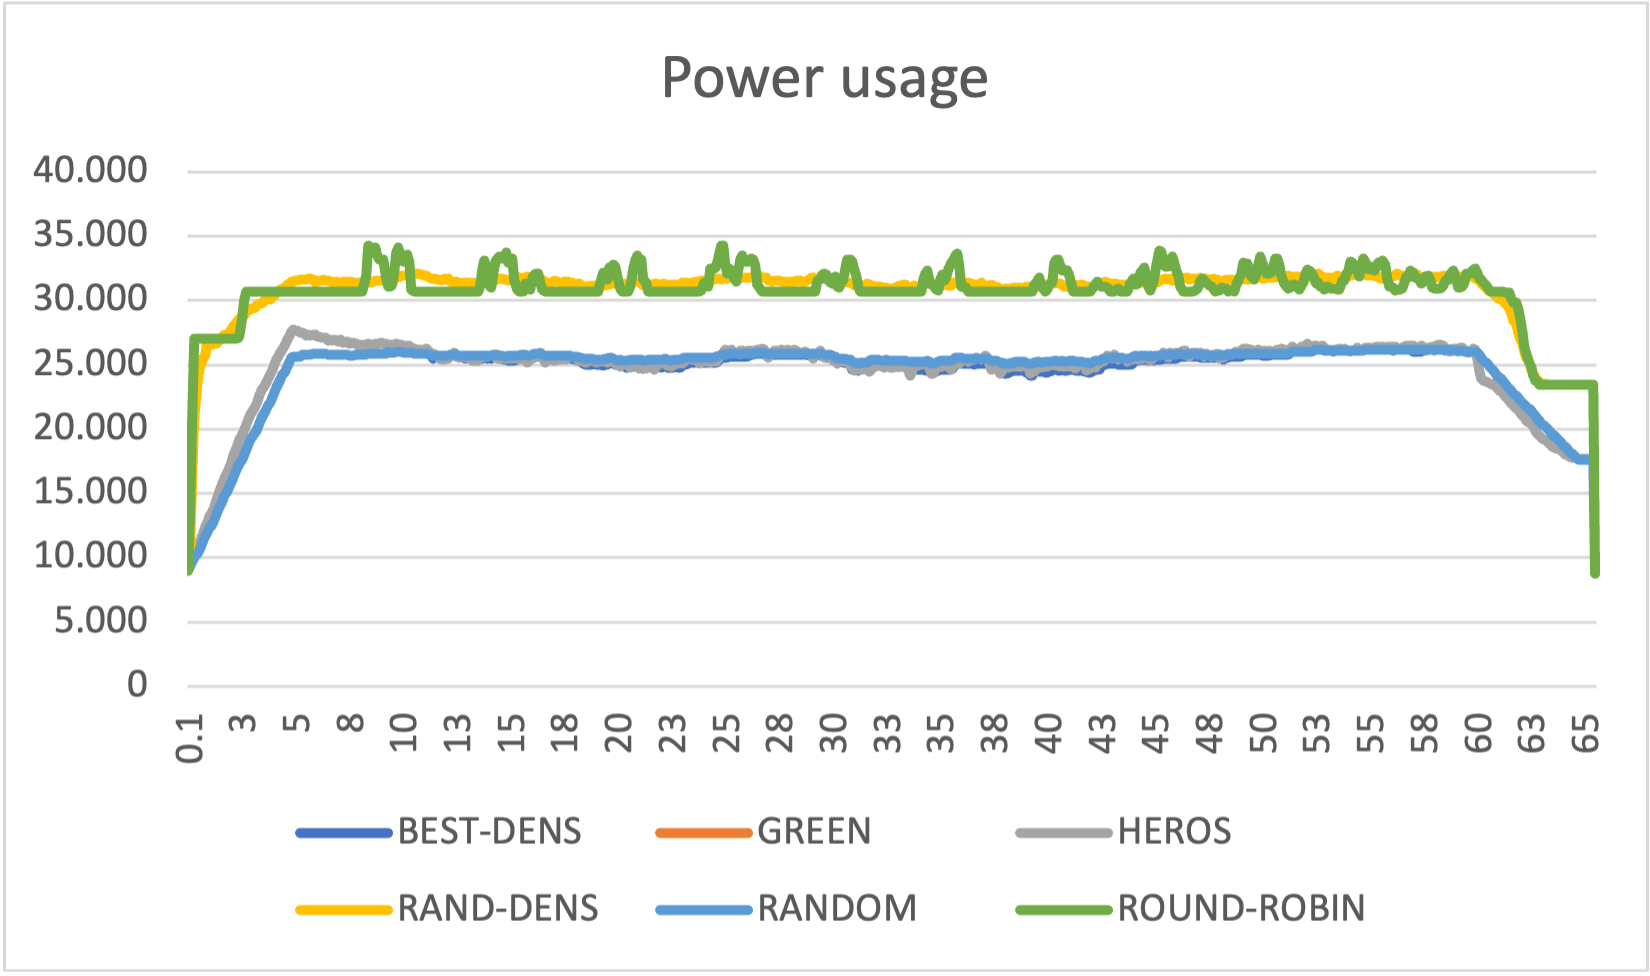
\includegraphics[width=0.7\textwidth]{chapters/images/schedulers_energyconsumption.png}
    \caption{Scheduling algorithms energy consumption}
    \label{fig:schedulers_energyconsumption}
\end{figure}

\begin{figure}[h]
    \centering
    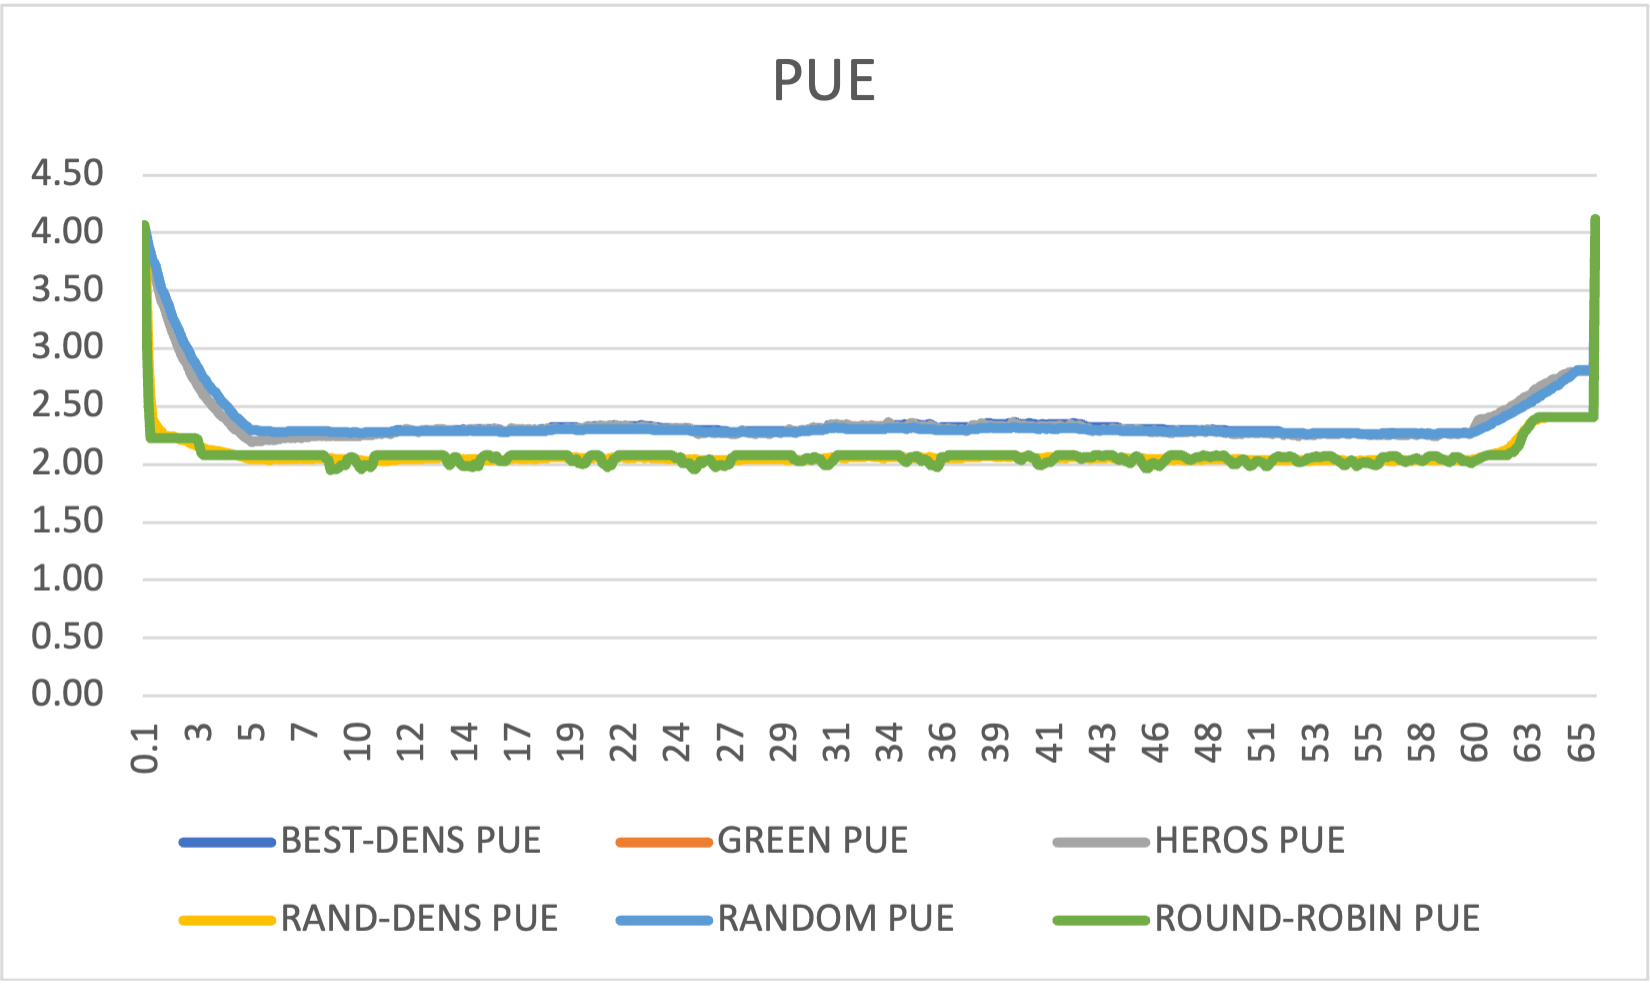
\includegraphics[width=0.7\textwidth]{chapters/images/schedulers_pue.png}
    \caption{Scheduling algorithms \emph{PUE}}
    \label{fig:schedulers_pue}
\end{figure}

\begin{figure}[h]
    \centering
    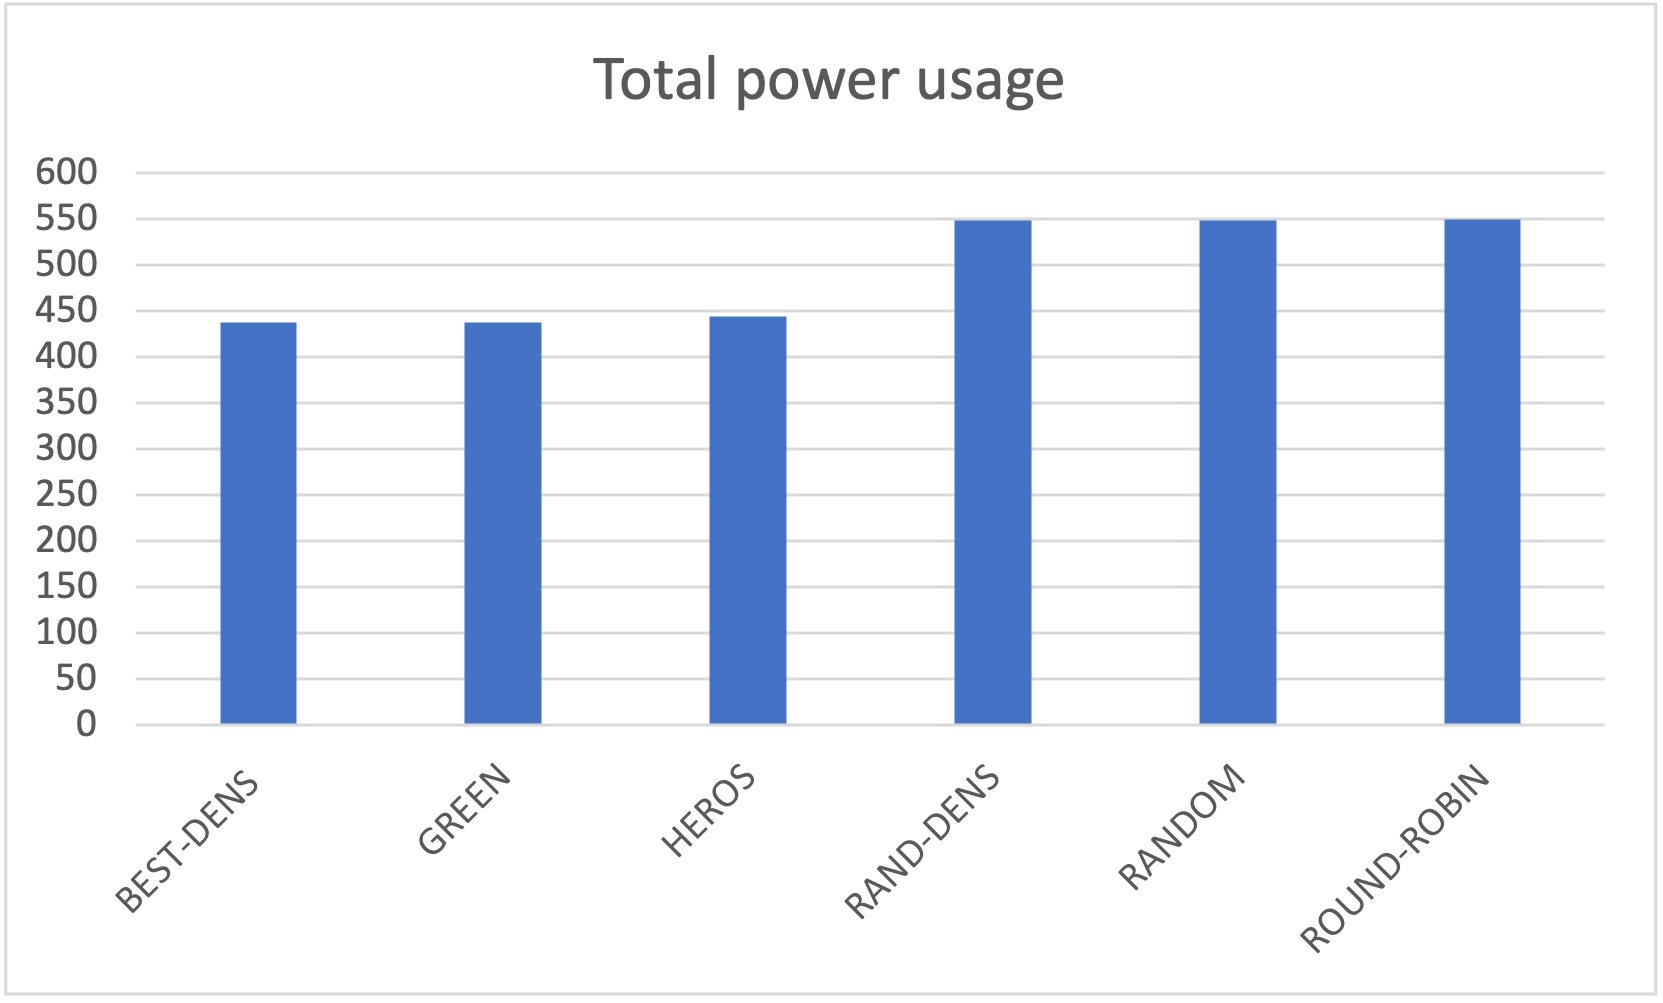
\includegraphics[width=0.7\textwidth]{chapters/images/schedulers_totalconsumption.png}
    \caption{Scheduling algorithms total power usage}
    \label{fig:schedulers_totalconsumption}
\end{figure}
As indicated by the charts, it is evident that the algorithms that perform better are \emph{BEST-DENS}, \emph{GREEN}, and \emph{HEROS} as they manage to achieve an energy-saving of approximately 22\% compared to the other three algorithms.

